\documentclass[11pt,a4paper]{article}
\usepackage[top=.75in, bottom=.1in, left=.75 in, right=.75in]{geometry}
\usepackage{graphicx}
\usepackage{natbib}
\usepackage{gensymb}
%\begin{footnotesize}
%\address{1300 Centre Street \\ Boston, MA, 20131}
%\end{footnotesize}
\begin{document}
\bibliographystyle{..//refs/styles/besjournals.bst}
\def\labelitemi{--}
\parindent=24pt
\includegraphics[width=0.2\textwidth]{/Users/danielbuonaiuto/Desktop/arb_logo.png}
\pagenumbering{gobble}
\\\\
{Dear Dr. Pinfield-Wells,}\\
\vspace{1.5ex}\\
\noindent We propose a ``Viewpoint" about the drivers of phenological sequences, focusing on flower-leaf sequences (FLSs), with implications for future plant communities. Evolutionary theory predicts that both flowering and leaf phenology are critical fitness components of woody plants, and a century of empirical research supports this assertion \citep{Munguia-Rosas2011,Forrest2010}. In recent decades, research has shown that it is not only individual phenophases but also the relationship between them that determines woody plant fitness \citep{Menzel1999,Ettinger2018}. Many deciduous woody plants flower before leafing, yet sustained research efforts have yet to yield a well-supported explanation for this. These unresolved hypotheses are important now as climate change is shifting FLSs---which may exacerbate fitness differences between species and reshape future ecosystems. Our ``Viewpoint" shows how progress in this area has been stalled by the current conceptual framework for FLSs; we detail a new approach that leverages continuous measures of FLSs and intra-specific and within-individual variation to rapidly advance progress.\\

\noindent \emph{What hypotheses or questions does this work address?}\\
% Nice opener!
\noindent Research suggests FLSs are under strong selection and critical to fitness. FLS variation may be an adaptation for wind-pollination \citep{Rathcke_1985}, reducing water stress \citep{Gougherty2018,Reich1984}, or early season flowering \citep{Primack1987}, but these conflicting hypotheses remain unresolved. A novel approach focusing on intra-specific FLS variation and quantitative comparisons is necessary to accurately evaluate these hypotheses.\\

\noindent \emph{How does this work advance our current understanding of plant science?}\\
\noindent We show: 1) The current framework fails to capture the inter- and intra- specific FLS variation in nature impeding robust hypothesis testing; 2) Variation provides novel insights about the function of FLSs, revealing complexities critical to advancing the hypotheses; 3) Leveraging intra-specific variation advances our understanding of FLSs.\\ % 'revealing consistencies and anomalies in support for the hypotheses' is a bit tricky to understand ... you could cut it, or replace with 'revealing complexities critical to advancing our understanding' or leave it.

\noindent \emph{Why is this work important and timely?}\\
\noindent We show that climate change is altering FLSs, but effects vary across species (0.8-4.7 days, Fig. \ref{fig:Figure 1}). Shifts could be beneficial or adverse, and predicting this outcome requires researchers to effectively evaluate the current hypotheses. Our framework is the first that can do this robustly, making it critical to fundamental and applied research.\\

 \noindent We expect this manuscript will be titled ``Reconciling competing hypotheses regarding flower-leaf sequences in temperate forests for fundamental and global change biology.'' It will be co-authored by I. Morales-Castilla, and E.M. Wolkovich. This proposed manuscript is not under consideration anywhere else. Thank you for your consideration.\\
\\Sincerely,\\\\\\\\\\

\noindent Daniel Buonaiuto\\

\newpage
\section*{Abstract:}
Phenology is a major component of an organism's fitness. While individual phenological events affect fitness, growing evidence suggests that the relationship between events may be equally or more important. This may explain why deciduous woody plants exhibit considerable variation in the order of reproductive and vegetative events, or flower-leaf sequences (FLSs). Research suggests that FLSs are adaptive, with several competing hypotheses to explain their function. Reconciling these hypotheses has been impeded by how FLS patterns are described and defined. Here, we advance the existing hypotheses to account for the FLS variation in nature and evaluate them with four case studies. Our inquiry provides three major insights towards a new framework for understanding FLSs. First, we find concurrent support for multiple hypotheses, suggesting progress can come from studies addressing overlapping hypotheses. Second, support for FLS hypotheses is sensitive to how FLSs are defined, with quantitative definitions proving most useful. Finally, we indentify the limits of trait-based hypothesis testing. We highlight how adopting an intra-specific approach and evaluating fitness consequences of FLS variation could quickly determine the major drivers, with cascading benefits to improving predictions of how climate change will alter FLSs and thereby re-shape plant communities and ecosystems. 
\section*{Selected Figures:}
   \begin{figure}[ht!]
   \centering
 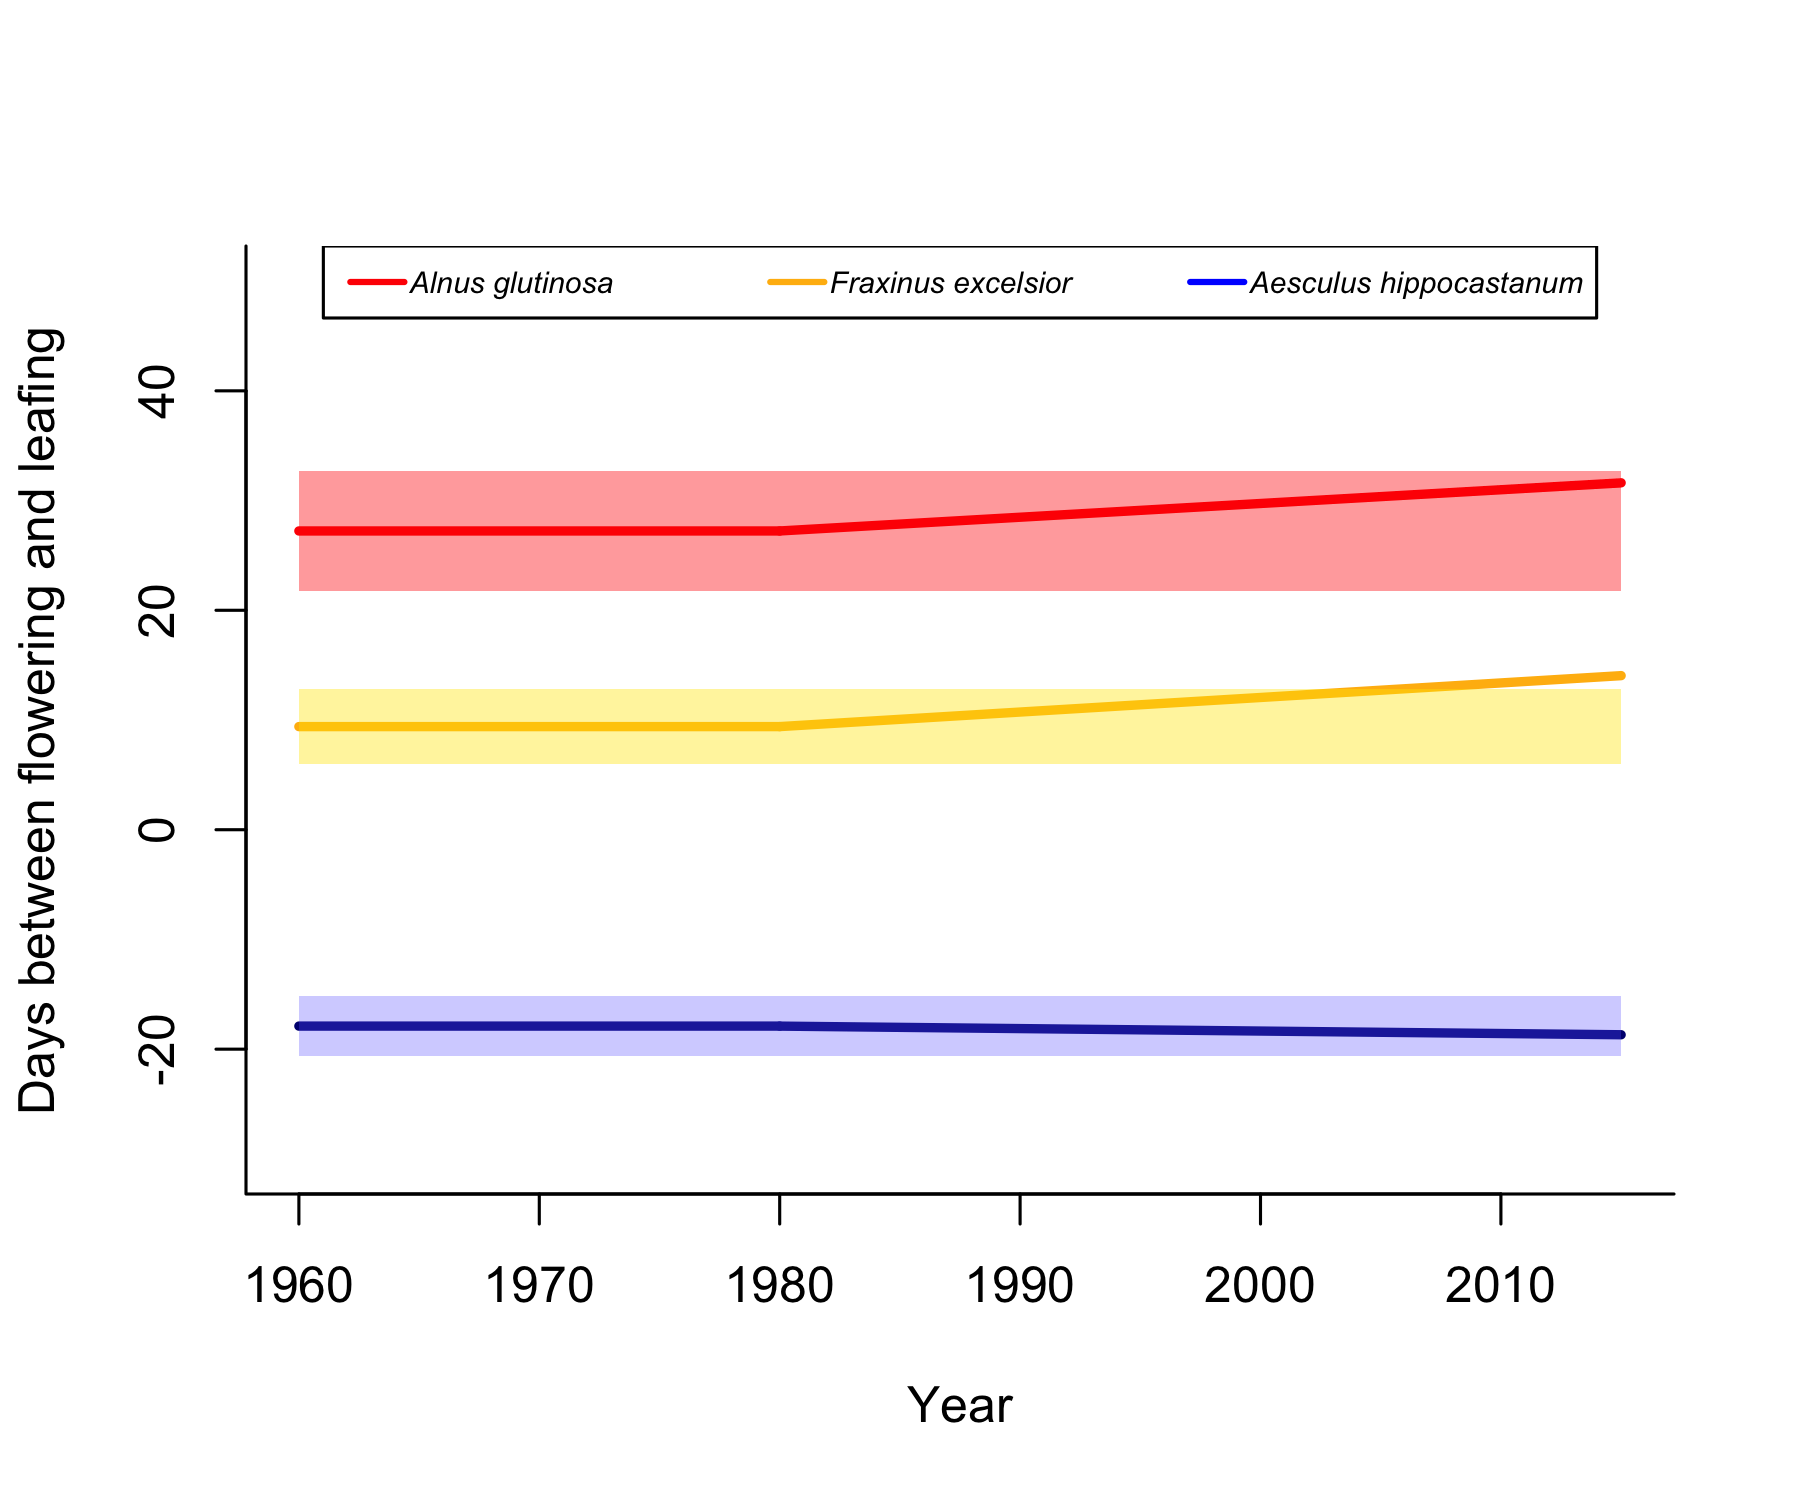
\includegraphics[width=.9\textwidth]{..//figure/FLS_climate_change.png}\\
\caption{\textbf{FLSs across Europe for three tree species from 1960 to 2015 suggests climate change has generally increased the time between flowering and leafing}, but the direction and rate of change differs across species, which may exacerbate fitness differences within forest communities. To detect the effect of climate change on average FLS, we used models that allow for shifts in FLS after 1980. Lines represent the mean trend in FLS per species, and the highlighted regions indicate historic range of FLS variability (upper and lower 95\% credible intervals of the pre-1980 average) from the PEP725 database \citep{PEP725}.}
    \label{fig:Figure 1}
    \end{figure}
\newpage
\bibliography{..//refs/hyst_outline.bib}

\end{document}